%describe the tasks to be completed that will satisfy the given objective
\section{Activity}

\subsection{Research}
Research the the MediaPlayer and MediaRecorder classes and methods. List which methods you believe will be crucial in programming the alarm system.

\subsection{Explore}
Open the AlarmSystemActivity.java file. Explore the file. Read the comments. Note the parts of the code that you will be required to fill in. They will be labeled.

\subsection{Import}
In order to use the classes and methods from APIs, you have to import the required libraries. Import the MediaPlayer and MediaRecorder libraries by inserting the following code at the beginning of the code below the other imports:
	
\begin{center}

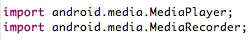
\includegraphics[scale=1]{imports.png} 

\end{center}


\subsection{Create}
Now we will create the media class instances and set them to null:\\

\begin{center}

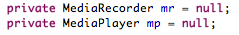
\includegraphics[scale=1]{instances.png} 

\end{center}

\noindent	
And then instantiate them in the onCreate method:\\

\begin{center}

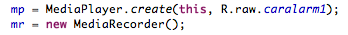
\includegraphics[scale=1]{instantiate.png} 

\end{center}

\noindent
The MediaPlayer instance (mp) is created with its context set to this and its loaded sound set to Sound 1 (R.raw.caralarm1).

\subsection{Sound Alarm Programming}
Now, let's program the buttons to sound the alarm. When the speaker button or sound alarm button is clicked, we want to play or stop the sound depending on if the alarm is already sounding. To do this, we will use the isPlaying() method in the MediaPlayer class to determine if (mp) is currently playing.\\

\begin{center}

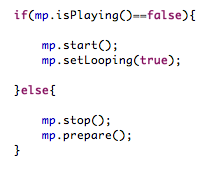
\includegraphics[scale=1]{ifelseSound.png} 

\end{center}

\subsection{Activate Research}
Next, we will program the activate button. This will be done in the listen method of the code. There are 4 functions in the MediaRecorder instance that must run before it can start recording. Research how MediaRecorder works and determine what these 4 functions are. Provide the link to the site where you found the information.

\subsection{Activate Programming}
Now, that you know what these 4 functions are and what they do, let's code:\\

\begin{center}

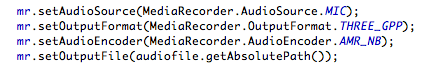
\includegraphics[scale=1]{mediaRecorder.png} 

\end{center}

\noindent	
The output file uses a file declared earlier in the code. You do not need to worry about this file. It has already been coded.

\subsection{Record}
With the MediaRecorder (mr) ready to record, now let's start recording:\\

\begin{center}

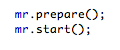
\includegraphics[scale=1]{startRecord.png} 

\end{center}

\noindent
Research the prepare method. Why does it have to be called before start the recorder?

\subsection{Analyze}
Next, we will analyze the recorded audio to determine if the amplitude has reached a certain point. Which method in the MediaRecorder class do you think would be helpful in achieving this?\\

\noindent
In order to accomplish this, we will set up a loop that continually checks the maximum amplitude reached, and then check it against the threshold we set up:\\

\begin{center}

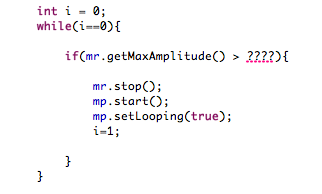
\includegraphics[scale=1]{amp.png} 

\end{center}

\noindent
Everything is now coded except for the amplitude threshold to check for. Test this number and determine which amplitude will be the best. You can research the range this value can be.

\subsection{Summary List}
The alarm system should now be working properly. Create a list of all the methods used from the MediaPlayer and MediaRecorder libraries with a description of what the method does and what it accomplished in the program.